\section{Architecture and rationale of EPS}
\label{sec:EPS_architecture_rationale}

\subsection{Available alternatives}
\label{subsec:available_alternatives}

The endeavour that Juno faces to generate enough electricity to sustain science operations at approximately 5.45 AU required particular attention in designing an efficient and reliable electric control system. Particularly, different options were present to generate the amount of power required, each of them with advantages and disadvantages:

\begin{itemize}
    \item \textbf{RTG:} the choice of a radioisotope to generate electricity could be considered. To generate the amount of power required around Jupiter, during the planetary phase (\autoref{table:power_budget}), one RTG of the same size of the one present on board New Horizons spacecraft  would have been sufficient ($\approx$ 250 We of production at BOL).\cite{nh_rtg} Electric power requirement would also be lower as some heat could have been routed to the propulsion section to heat up the tanks and fuel lines. This choice however had some problems, mainly with respect to the safety during Earth EGA, radiation contamination, heat dissipation at distances lower than 2 AU from the Sun and weight distribution. Particular problems could have rose as the said RTG generates around 4.4 kW of heat, requiring a very efficient dissipation system for the first years of the mission, oversizing it with respect to the nominal orbit around Jupiter. Availability of Plutonium-238 was also critical as suppliers could not guarantee the needed amount of fuel with the needed power output, given the stop in the production of the said isotope during the 80s.\cite{plutonium}
    
    \item \textbf{Solar panels:} no spacecraft equipped with solar panels has ever been tested at 5.45 AU from the Sun. This choice would have required a very large surface area, and thus precautions had to be taken into account inside the fairing during launch operations, to provide enough power for safe operations at Jupiter. A complex management system is also required in order to not discharge too much current inside the electronics during the ICs and the OC as the amount of solar flux hitting the S/C during different parts of the mission dramatically reduces. More stringent pointing requirements are also present as not having a clear view of the Sun could have led to the need of bigger and heavier batteries.
\end{itemize}

Considering also the driving requirement of utilizing as much as possible off the shelf components, budget constraints, the limited supply of plutonium and the different possible configurations offered, solar panels were chosen. This choice led to a particular design of the satellite, where mass distribution was exploited to grant more stability throughout the different phases of the mission.  

\subsection{Components and distribution}
\label{subsec:components_and_distribution}

The flown spacecraft is fitted with 3 solar arrays as the primary source and 2 Li-Ion batteries as the secondary one. SASU are used to manage the generated power and a PDDU is responsible of managing and distributing electricity to the various subsystems.
The whole system works at 28 V DC, which is a standard for low-power consumption system as Juno.

\subsubsection{Solar arrays}
\label{susubsec:solar_arrays}

The arrays are mounted on the side of the main body, spaced 120° apart, and are composed by a different number of panels: A1 presents only 3 panels while A2 and A3 present 4 panels each. The total mass of the arrays is 340 kg, with a total area of 60 m$^2$ \cite{arrays_mass} and an active area of 49.77 m$^2$, composed by 18.698 solar cells.\cite{masses_ref} 
Each cell, produced by Spectrolab \cite{solar_datasheet}, is in an UTJ configuration, to obtain optimum packing and high performances in LILT environments like the one around Jupiter. The three layers, Ge for the bottom cell, GaAs for the middle cell and GaInP$_2$ for the top cell, are placed on top of a Germanium Kapton substrate and connected with tunnel junctions. A multi junction configuration optimizes the electromagnetic spectrum exploitation, focusing on specific wavelength bands. An anti-reflective Si coating protects the cell from the harsh environment of Jupiter. 

 Solar panels are linked one to the other and to the main body with electro-actuated hinges and the first panel of each array is supported by struts. All these elements are needed to both extend the panels soon after separation from the Centaur and to control the position of the arrays during all the operations. This is necessary to take into account the bending of the arrays during large manuevers and their thermal expansion. Moreover it is necessary to align the main inertia axis (Z-axis) with the spin axis due to the particular mass distribution of the panels and of the instrumentation. Power produced by each panel is varying in each phase, depending on incidence and distance from the Sun. Values at 1 AU are in the range of 14 kW and about 400 W EOL. This value consider all the  active surface to be working. Fixing the attitude of the spacecraft, as the distance increases, and thus the solar flux decreases, a lower current is produced at the same voltage. However with the increase of distance, and thus the decrease of the temperature, the current decreases, the cells' efficiency increases and an higher voltage is produced. Cell efficiency at 28°C is 28.4\%.  Given that Juno's trajectory ranges between 0.88 AU and 5.45 AU from the Sun, the cells are grouped in strings of three different lengths, whose connection must be adjustable to satisfy power, voltage and current requirements in each phase. When not in use, the power generated by each cell is left on the panels to be dissipated as heat. This is crucial to ensure a high level of efficiency, increasing as temperature decreases, throughout the whole journey. The rationale for the distribution of the cells in each panel is shown in \autoref{fig:Solar panels reasoning} and explained as follows. 
\rfigII{Solar panels reasoning}{Cell distribution rationale}{0.55}{18}{-5mm}{-4mm}
Once fixed the cell type used for the whole mission and known the power, voltage and current required in each phase, exploiting the characteristic curve of each cell, the number of cells that must be connected in series and in parallel can be obtained and so the required string length type. Then, as the cells' dimension is known and the length of the required strings has been retrieved, the area of each string can be computed. The mass of the panels needs to be distributed so that the inertia matrix becomes as diagonal as possible, with the constraint that only one string type can be fitted in each panel. Indeed in the case of a panel composed by all three types of strings, hot spots due to the activation of only a single type of string could lead to uneven internal stresses and thus damaging the whole panel. Moreover, damages to a single panel in this case would lead to the loss of multiple types of strings, reducing the available power during different phases of the mission.  However, given all the aforementioned requirements and considering also the limited amount of space inside the Atlas V's fairing, A3P1 had to feature both medium and short strings. The resulting string configuration is reported in \autoref{table:strings_description}. The maximum number of strings in parallel and the minimum activation distance are limits that ensure the survivability and correct operation of the system: exceeding these limits, and thus generating a current above 7A, would blow the fuse on that string, compromising the whole mission. The critical points of the mission to prevent middle string turn on is 1.2AU $\div$ 1.5AU and 1.5AU $\div$ 1.9AU for short strings.

 \begin{table}[H]
    \renewcommand{\arraystretch}{1.3}
    \centering
    \small
\begin{tabular}{|c|c|c|c|c|}
    \hline
    \textbf{String type} & \textbf{\# cells in series per string} & \textbf{\# strings} & \textbf{Max \# strings in parallel} & \textbf{Minimum distance [AU]}\\
    \hline
    \hline
    \textbf{Long}    &  22 & 114 & - & 0.88 \\
    \hline
    \textbf{Medium}  &  14 & 369 & 40 & 1.8\\
    \hline
    \textbf{Short}   &  13 & 848 & 64 & 3.8 \\
    \hline
\end{tabular}
\caption{Strings description}
\label{table:strings_description}
\end{table}

\vspace{-3mm}

Consequently, as can be seen in \autoref{table:panels_area} and \autoref{table:panels_mass}, A2P1, A2P2 and A2P3, and the same in A3, are slightly smaller than the A1 correspondents while the presence of A2P4 and A3P4 counterbalances the presence of the MAG boom on the tip of A1.

\vspace{3mm}

\begin{minipage}{0.4\linewidth}
    \centering
    \captionsetup{type=figure}
    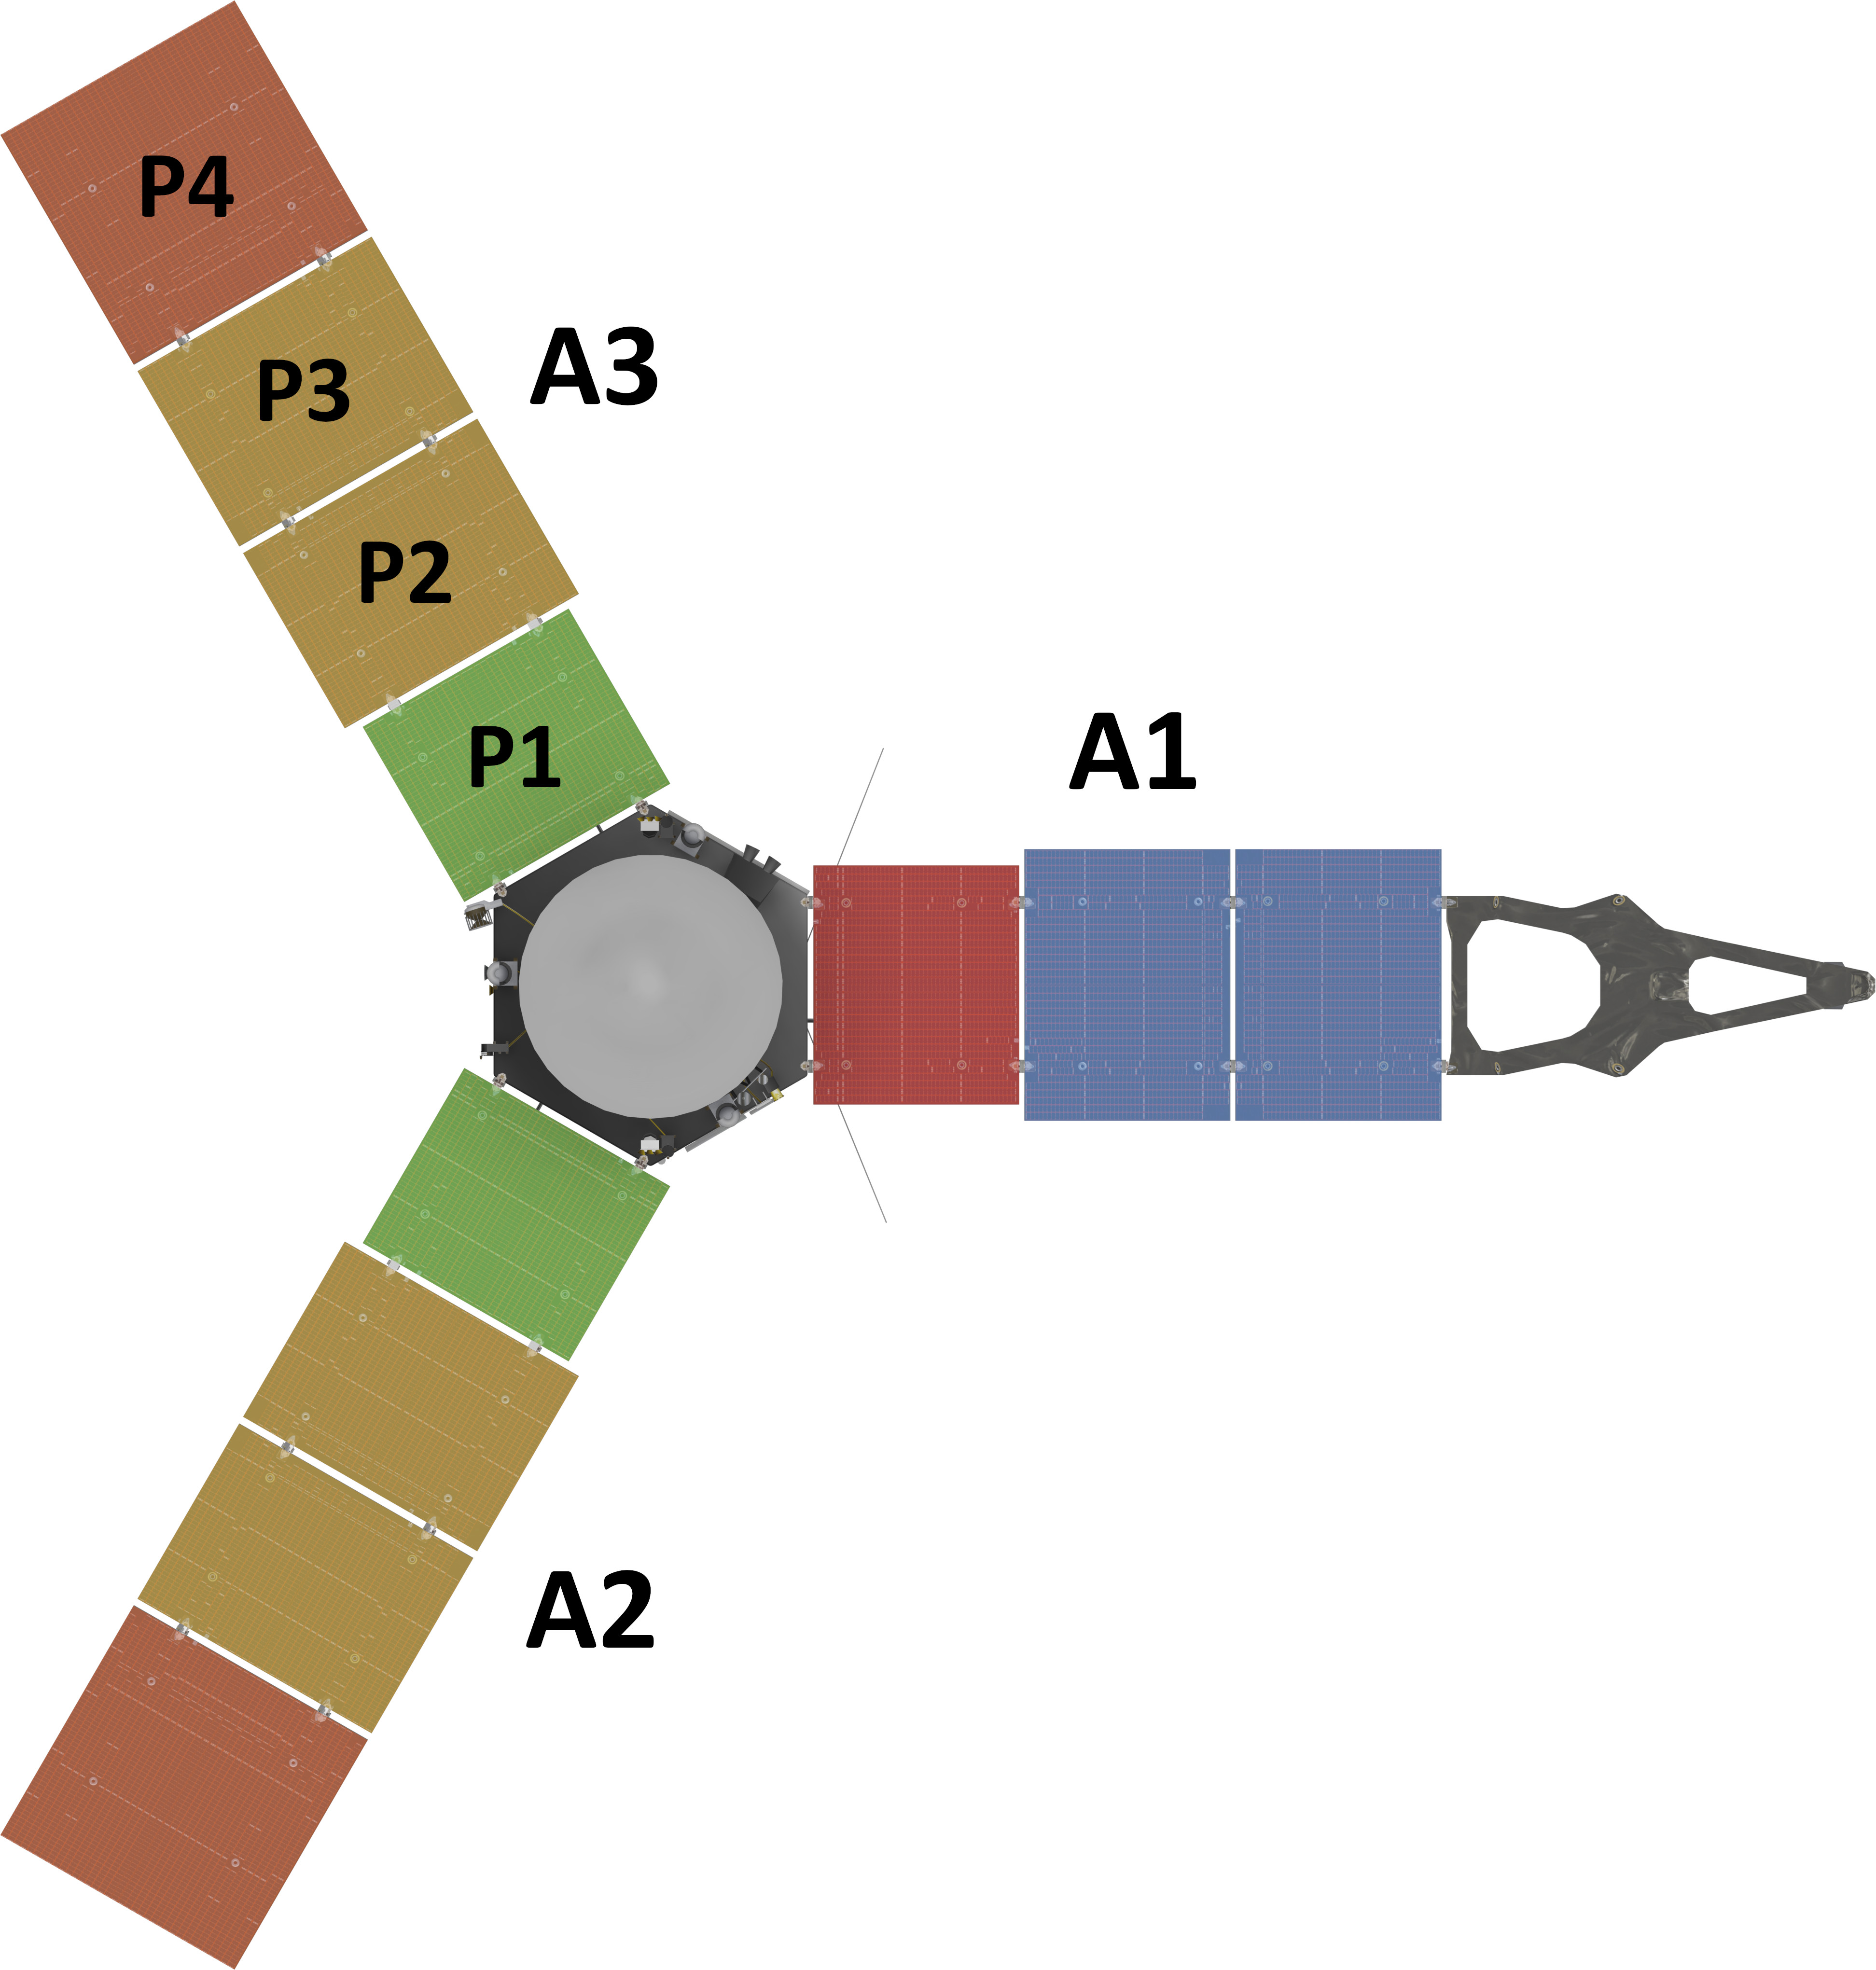
\includegraphics[width=\linewidth]{Images/Juno panels.jpg}
    \caption{Juno's panel configuration}
    \label{fig:panel_config}
\end{minipage}\hfill
\begin{minipage}{0.5\linewidth}
    \centering
    \small
    \captionsetup{type=table}
    \renewcommand{\arraystretch}{1.4}
    \begin{tabular}{|c|c|c|c|c|c|}
        \hline
        &  \textbf{P1}  & \textbf{P2} & \textbf{P3} & \textbf{P4} & \textbf{Array's area} \\
        \hline
        \hline
        \textbf{A1}      & 4.92 & 5.60 & 5.60 & - & 16.11  \\
        \hline
        \textbf{A2}      & 4.81 & 5.46 & 5.46 & 6.29 & 22.02 \\
        \hline
        \textbf{A3}     & 4.81 & 5.46 & 5.46 & 6.29 &  22.02 \\
        \hline
    \end{tabular}
    \caption{Panels areas [m$^2$]}
    \label{table:panels_area}

    \vspace*{5mm}

    \begin{tabular}{|c|c|c|c|c|c|}
        \hline
        &  \textbf{P1}  & \textbf{P2} & \textbf{P3} & \textbf{P4} & \textbf{Array's mass}\\
        \hline
        \hline
        \textbf{A1}      & 27.81 & 31.62 & 31.62& - & 91.05 \\
        \hline
        \textbf{A2}      & 27.17 & 30.89 & 30.89 & 35.54 & 124.47 \\
        \hline
        \textbf{A3}     & 27.17 & 30.89 & 30.89 & 35.54 & 124.47 \\
        \hline
    \end{tabular}
    \caption{Panels masses [kg]}
    \label{table:panels_mass}
\end{minipage}

% ----- dobbiamo inserire  la radiazione incidente ------

\subsubsection{Batteries}
\label{subsubsec:Batteries}
Juno is equipped with two Li-Ion batteries in cold redundance: these ensure complete operability throughout the whole mission, even when the power generated by the solar panels is not sufficient.
The mounted batteries are produced by EaglePicher, a proven and already flown design\cite{batteries_juno}. Particularly each of the two cells is able to hold up to 55 Ah in a range between 24.0 V to 32.8 V. Voltage at 50\% SoC is 29.4 V.\cite{solar_panels_coef} The choice of Lithium Ions batteries is related to their high energy density, longevity (as Juno mission had to last at least 7 years), limited self discharge, higher number of cycles and wider range of operating temperatures with similar DoDs with respect to other types of batteries.
This battery is characterized by a particular high value in terms of specific power as its primary usage is to cover the peaks of the system during science operations.
The total mass for the batteries, without considering the applied MLI and radiation shielding is about 32 kg, 16 kg each. Considering that the available datasheet \cite{batteries_juno} is not the one for Juno mission but for MAVEN, a mission around Mars with various cycles of sunlight and eclipses, a significant difference in the DoD and life cycles must be made: Juno's trajectory was carefully planned to avoid as much as possible eclipses, with the exception of EGA. The batteries are more than capable to handle that $\approx$ 19 minutes eclipse \cite{juno_inner} and are heavily used to perform science operation around Jupiter, when the power request exceeds of about 110 W the power generated by the solar arrays.

\rfigII{Juno batteries}{Position of the 2 batteries (red box)}{0.4}{18}{-7mm}{-7mm}


This design mission required 33 science orbits around Jupiter, one EGA and a total of four manuevers where Juno's panels did not face directly the Sun: the cycles the batteries have to sustain is much lower than the 40.000 cycles at 40\% DoD of MAVEN. This difference allowed to discharge more the batteries and thus to reduce the weight of the system while guaranteeing its correct operability. Since the mission is still ongoing seven years after its planned decommissioning, as a consequence of the numerous failures of the propulsion system which did not allow to perform the critical PRM, the sturdiness and effectiveness of the batteries as the generated power from the solar panels is lower than the planned EOL one is proven. Given the previously described limits of Amperes the system is capable to handle, the batteries are charged at C/50 and continuously kept at 50\% SoC during ICs and OC and only charged to the needed percentage prior to the manuever. Different panels' strings are capable of reaching the correct voltage to charge the batteries at 50\% SoC and beyond, in particular the middle strings from 1.2 AU and the short strings from 1.5 AU from the Sun. Full charge voltage of the said string is reached at 1.5 AU and 2.5 AU respectively, while long strings are capable to fully charge the batteries at closer distance from the Sun as they are the first to be turned on. Strings can provide the needed voltage sooner than required, but the described safety procedure in \autoref{susubsec:solar_arrays} must be taken into account.\cite{solar_panels_coef} The positioning of the batteries is critical given the harsh environment Juno faces: temperature range for the on board batteries is tighter than the solar panels' one. The latter are rated to work between -133 °C and +96 °C, the batteries instead are only capable to withstand temperatures between -20°C to +40°C. As the batteries are mounted on top of the propulsion module, and linked to all the instruments by external and shielded cables, on the exterior of the S/C, they need to be protected thermally, while they are rated to withstand the predicted radiation along Juno's orbit around Jupiter.\cite{batteries_position} A MLI blanket over a Beryllium box is present to help the heaters keeping the batteries inside their operating range. Given the size of the batteries, 30.1 cm $\times$ 20.56 cm $\times$ 23.85 cm each, they could not be placed inside the vault, where all the electronics is positioned: dimension needed for the vault (now at  $\approx$ 80 cm $\times$ 80 cm $\times$ 70 cm ) would have almost doubled and thus its mass would have been significantly higher, at over 200 kg.\cite{batteries_position}

\subsubsection{Power distribution}
\label{subsec: pwr_distribution}

The EPS of Juno handles the generation of power from the solar array  in order to cope with the large Sun range variation. Before 2000s, few missions were capable to produce such energy with merely solar panels. The increased efficiency of solar cells technology, reliability and methods to cleverly rearrange cell strings configuration have allowed the access of this technology also to deep space missions such Juno. 
Due to lack of information about the primary source distribution method, the Solar Array Switching Unit (SASU) patent developed by Nasa and Lockheed Martin in 1998 was assumed to be the one used. \cite{sasu}
As previously said, the need to have three different strings is driven by the different radiation and temperature conditions encountered along the mission that change the performances of the cells. The patent of the SASU comes from the need to manage in a clever way the power generation, in order to furnish always a constant voltage to the main bus and fulfil the power demand of the subsystems. The switching unit is composed by:
\begin{itemize}
    \item switch circuits to connect the strings as imposed by the control system;
    \item the control system;
    \item external shunt power card, which shunts the excess of power generated;
\end{itemize}

The bus voltage is battery-regulated, which means that no BCR nor BDR are present on-board. \cite{bat_regulator}
This design choice is typical for NASA unmanned spacecrafts. \cite{systems_book}
The absence of a dedicated regulator improves the efficiency and lowers the mass of the system.
The PDDU is responsible for delivering the required power to all the loads which are then self-regulated in order to generate the required tension and current. This is particularly true for the some of the on-board instruments: for example JEDI\cite{JEDI_info} and JADE\cite{JADE_info} require voltages up to 10 kV while the MAG\cite{MAG_info} suite requires AC current to safely conduct measurements.